\documentclass[a4paper,14pt]{extreport}
\usepackage[T2A]{fontenc}
\usepackage[utf8]{inputenc}
\usepackage[russian]{babel}
% величины отступов:
\usepackage[left=2.5cm, right=1.5cm, top=2.5cm, bottom=2.5cm]{geometry}
\usepackage{alltt}
\usepackage{graphicx}
\graphicspath{{img/}}

\usepackage{titlesec}
\titleformat{\chapter}[block]
{\normalfont\Large\bfseries}{\thechapter}{0.5em}{\Large}



\titleformat{\section}
{\normalfont\bfseries}{\thesection}{0.5em}{}

\titlespacing*{\chapter} {0pt}{\baselineskip}{20pt}

\titlespacing*{\section} {0pt}{\baselineskip}{10pt}


\titleformat{\subsection}
  {\normalfont\bfseries}
  {\thesubsection}
  {0.5ex}{}

\titlespacing*{\subsection} {0pt}{\baselineskip}{5pt}

\usepackage{titletoc}

\titlecontents{chapter}
[0pt]
{}
{\contentsmargin{0pt}
    \thecontentslabel\enspace
    \large}
{\contentsmargin{0pt}\large}
{\titlerule*[.5pc]{.}\contentspage}
[]  

\usepackage[hidelinks]{hyperref} % гиперссылки в содержании

\begin{document}
%----------ТИТУЛЬНЫЙ-ЛИСТ--------------
	\center
	Министерство образования Республики Беларусь\\
	Учреждение образования «Белорусский государственный университет информатики и радиоэлектроники»
	\vspace*{2cm}
	\endcenter
	\raggedright
	Факультет компьютерных систем и сетей\\
	\medskip
	Кафедра программного обеспечения информационных технологий\\
	\vspace*{2cm}
	\center
	ПОЯСНИТЕЛЬНАЯ ЗАПИСКА\\
	к курсовому проекту по дисциплине: Объектно-ориентированное программирование\\
	на тему:\\
	\medskip
	"Библиотека chart"\\
	\vspace*{4cm}
	\endcenter
	\raggedright
	\hspace*{7.94cm}Выполнил:\\
	\hspace*{7.94cm}студент гр. 251005 Кастюк А.В.\\
	\bigskip
	\hspace*{7.94cm}Руководитель: асс. Третьяков Ф.И.\\
	\center
	\vspace*{6cm}
	Минск 2015
	\pagestyle{empty}
%-------ЛИСТ-ЗАДАНИЯ--------------
	\newpage
	\center
	Учреждение образования\\
	\medskip
	«Белорусский государственный университет информатики и радиоэлектроники»\\
	\medskip
	Факультет компьютерных систем и сетей\\
	\medskip
	\endcenter
	\raggedright
	\hspace*{9.53cm}УТВЕРЖДАЮ\\
	\hspace*{9.53cm}Заведующий кафедрой ПОИТ\\
	\hspace*{9.53cm}\underline{\hspace{6cm}} \\
	\hspace*{11cm}\small (подпись) \normalsize\\
	\hspace*{9.53cm}\underline{\hspace{5cm}}2015 г.\\
	\medskip
	\center
	ЗАДАНИЕ\\
	по курсовому проектированию\\
	\medskip
	\endcenter
	\raggedright
	Студенту \underline{Кастюку Алексею Валерьевичу}\\
	\begin{enumerate}
	\item Тема работы \underline{Библиотека chart}\\ 
	\item Срок сдачи студентом законченной работы \underline{09.06.2015}
	\item Исходные данные к работе \underline{Среда разработки Sublime text 2. }
	\item Содержание расчётно-пояснительной записки (перечень вопросов, которые подлежат разработке)\\
	\underline{\hspace*{16cm}}\hspace*{-16cm}Введение. 2. Постановка задачи. 3.Разработка программного средства.\\
	\underline{\hspace*{16cm}}\hspace*{-16cm}4. Тестирование программного средства. Руководство пользователя.\\
	\underline{\hspace*{16cm}}\hspace*{-16cm} Заключение. Список используемой литературы. Приложения.\\
	\item Перечень графического материала (с точным обозначением обязательных чертежей и графиков)\\
	\underline{1. Схема алгоритма}
	\item Консультант по курсовой работе\\
	\underline{Третьяков Ф.И.}  
	\item Дата выдачи задания \underline{12.02.2015}
	\item Календарный график работы над проектом на весь период проектирования (с обозначением сроков выполнения и процентом от общего объёма работы):\\ 
	\underline{\hspace*{16cm}}\hspace*{-16cm}разделы 1, 2, 3 к 05.03.2015 – 30 \% готовности работы;\\ 
	\underline{\hspace*{16cm}}\hspace*{-16cm}раздел 4 к 02.04.2015 – 60 \% готовности работы;\\
	\underline{\hspace*{16cm}}\hspace*{-16cm}раздел 5, 6 к 20.05.2015  –  90 \% готовности работы;\\
	\underline{\hspace*{16cm}}\hspace*{-16cm}оформление пояснительной записки и графического материала к\\
	\underline{\hspace*{16cm}}\hspace*{-16cm}08.06.2015 – 100 \% готовности работы.\\
	\underline{\hspace*{16cm}}\hspace*{-16cm}Защита курсового проекта с 01 по 09 июня 2015 г.\\
	\end{enumerate}
	\hspace*{7cm}РУКОВОДИТЕЛЬ\underline{\hspace*{6cm}}\hspace*{-3.9cm}Третьяков Ф.И.\\
	\hspace*{11.5cm}\small (подпись) \normalsize\\
	\bigskip
	Задание принял к исполнению \underline{\hspace*{10.5cm}}\hspace*{-8cm}Кастюк А.В. 12.02.2015г.\\
	\hspace*{7cm}\small (дата и подпись студента) \normalsize\\
%-------СОДЕРЖАНИЕ--------------
\newpage
\pagestyle{plain}

\renewcommand\contentsname{СОДЕРЖАНИЕ}
\tableofcontents
\endcenter

%------Введение--------------
\newpage
\addcontentsline{toc}{chapter}{Введение}
\chapter*{Введение}
\hspace{4ex}В рамках данного курсового проекта необходимо разработать библиотеку для отображения данных в виде графиков и диаграмм на веб-странице.\\
\hspace{4ex}Многие веб-разработчики время от времени сталкиваются с необходимостью визуализировать сравнительно большое количество данных при помощи диаграмм, что позволяют наглядно и доступно донести информацию до пользователя. Раньше подобные графики делали в Excel, а затем вставляли на сайт картинкой. Но, в виду современных библиотек и возможностей языков программирования веб-приложений, такой метод не является оптимальным.\\

%------Постановка задачи--------------
\newpage
\chapter{Постановка\enspaceзадачи}
\hspace{4ex}Реализовать библиотеку для отрисовки графиков с помощью библиотеки D3.js, с помощью которой возможно отобразить следующие виды графиков и диаграмм:
\begin{enumerate}
	\item График
		\begin{itemize}
		\item Точки
		\item Линии 
		\item Сплайны
		\end{itemize}
	\item Круговая диаграмма
	\item Гистограмма
	\item Объемная круговая диаграмма
	\item Объемная кольчатая диаграмма
\end{enumerate}
\newpage
\chapter{Разработка\enspaceпрограммного\enspaceсредства}
\section{Обоснование\enspaceвыбора\enspaceинформационных\enspaceтехнологий}
\hspace{4ex}Для разработки данной библиотеки был выбран язык Javascript. Данный язык поддерживается всеми современными браузерами на всех операционных системах, что означает что приложение, написанное на Javascript, возможно запустить на любой платформе.\\
\section{Используемые\enspaceсредства\enspaceразработки}
\hspace{4ex}Вспомогательным элементом при написании проекта является библиотека D3.js, которая вне всякого сомнения, дарит много полезных возможностей, которых не хватает большинству существующих библиотек. Такие возможности как “Enter and Exit”, мощные переходы, и синтаксис, схожий с jQuery или Prototype, делают его одной из лучших JavaScript библиотек для создания графиков и диаграмм. В D3.js они генерируются посредством HTML, SVG и CSS. D3.js не работает должным образом со старыми браузерами, такими как IE8. Но разработчик всегда может применить такие плагины как \textit{aight plugin} для кроссбраузерной совместимости.

\hspace{4ex}Для написания кода программы будет использован текстовый редактор Sublime Text 2. Данное преложение является условно бесплатным и главное его приемущество --- большое количество плагинов и расширений для удобного создания кода программы.
\section{Разработка\enspaceпрограммного\enspaceсредства}
\hspace{4ex}Данный раздел подробно описывает функцианальность библиотеки и является руководством по разработке.
\subsection{Запуск\enspaceотрисовки\enspaceграфиков\enspaceна\enspaceстранице}
\hspace{4ex}Данная функция запускается при загрузке страницы и при изменении размера страницы.
\begin{verbatim}
window.onload = start;
window.onresize = function() {
    d3.selectAll("chart").select("svg").remove();
    d3.selectAll("chart").select(".tip").remove();
    start();
}

function start() {
    d3.selectAll("chart")
        .append('svg')
        .append('g')
        .attr('class', 'legend');
    d3.selectAll('chart').append('div').attr('class', 'tip')
    .html("<div class='s'></div><div class='p'></div>")
    d3.selectAll('chart')[0].forEach(function(val) {
        series(d3.select(val));
    });
};
\end{verbatim}
\begin{figure}[h]
\center{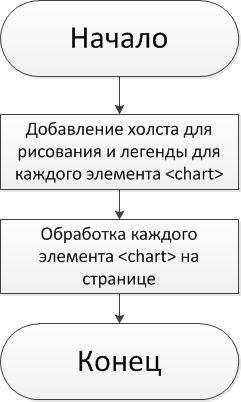
\includegraphics{start.png}}
\caption{Блок-схема функции запуска отрисовки графиков}
\label{ris:image}
\end{figure}
\subsection{Добавление\enspaceэлемента\enspaceв\enspaceлегенду}
\hspace{4ex}Данная функция предназначена для добавления названия элемента в легенду. Если имя пустое, то название запишется как 'serie'.
\begin{verbatim}
function legend_draw(legend, name, color, i) {
    var g = legend.append('g')
        .attr('transform', 
        'translate(0, ' + (i * 20 + 5 * i + 5) + ')')
    g.append('rect')
        .attr("width", 10)
        .attr("height", 10)
        .attr("fill", !color ? 'red' : color)
        .attr('x', 5)
        .attr('y', 5);
    g.append('text')
        .text(!name ? 'serie' : name)
        .attr('x', 20)
        .attr('y', 15);
}
\end{verbatim}
\begin{figure}[h]
\center{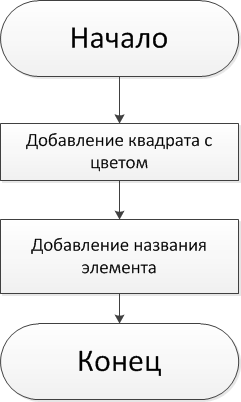
\includegraphics{legend_draw.png}}
\caption{Блок-схема функции добавления названия элемента в легенду}
\label{ris:image}
\end{figure}
\subsection{Обработка\enspaceэлемента\enspace<chart>\enspaceв\enspaceзависимости\enspaceот\enspaceтипа}
\hspace{4ex}Данная функция проверяет, какое значение аттрибута \textit{type} элемента <chart> присвоенно разработчиком для дальнейшего выбора условий отрисовки. Всего возможны варианты:
\begin{enumerate}
	\item \textit{undefined} (данное значение будет распозноваться библиотекой как значение "\textit{numeric}").
	\item \textit{numeric} (используется для отображения графиков). Также у данного типа есть свои виды отображения, которые могут сочетаться на одном графике:
	\begin{itemize}
		\item \textit{undefined} (данное значение будет распозноваться библиотекой как значение "\textit{point}").
		\item \textit{point} (отображает набор точек из данных из аттрибута \textit{data}).
		\item \textit{line} (отображает ломанную линию из данных из аттрибута \textit{data}).
		\item \textit{spline} (отображает плавную линию из данных из аттрибута \textit{data}).
	\end{itemize}	 
	\item \textit{pie} (используется для отображения круговых диаграмм).
	\item \textit{bar} (используется для отображения гистограмм).
	\item \textit{3d-pie} (используется для отображения объемных круговых диаграмм).
	\item \textit{3d-circle} (идинтичен \textit{3d-pie}, только с отверстием посередине).
	
\end{enumerate}
\begin{figure}[h]
\center{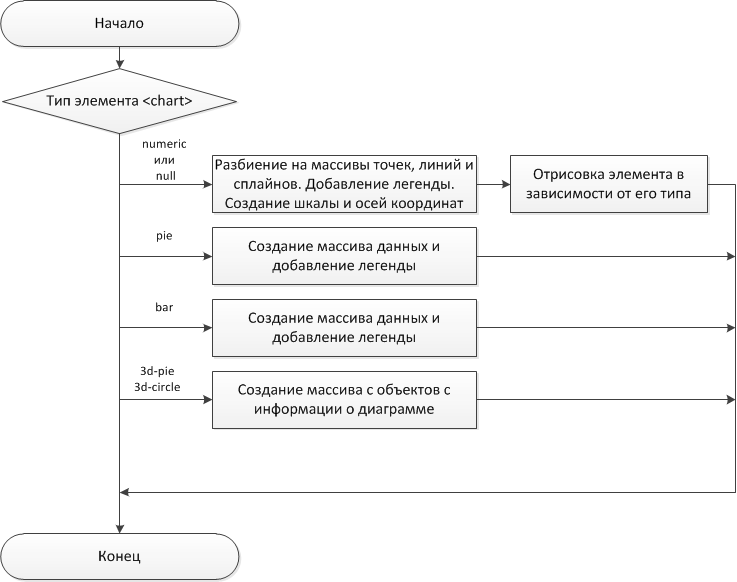
\includegraphics[scale=0.7]{series.png}}
\caption{Блок-схема функции обработки типа элемента <chart>}
\label{ris:image}
\end{figure}
\subsection{Получение\enspaceобласти\enspaceотображения\enspaceзначений\enspaceграфика}
\hspace{4ex}Функция предназначена для определения минимального и максимального значения для графика.
\begin{verbatim}
function getDomain(data, index) {
    var d = [];
    data.forEach(function(v) {
        v.forEach(function(v) {
            d.push(v[index])
        })
    });
    return [d.reduce(function(prev, next) {
            return Math.min(prev, next);
        }),
        d.reduce(function(prev, next) {
            return Math.max(prev, next);
        })
    ];
}
\end{verbatim}
\begin{figure}[h]
\center{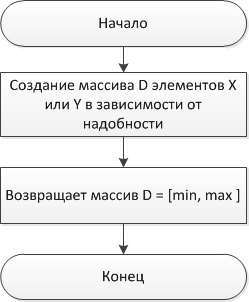
\includegraphics{getDomain.png}}
\caption{Блок-схема функции получения области отображения значений графика}
\label{ris:image}
\end{figure}
\subsection{Получение\enspaceмассива\enspaceзначений\enspaceдля\enspaceграфиков}
\hspace{4ex}Главной задачей данной функции является выделение всех включений шаблона "[число число]" и преобразование полученных данных в массив.
\begin{verbatim}
function getPointData(seriesSet) {
    var data = [];
    seriesSet.forEach(function(val) {
        data.push(
            val.attr('data')
            .match(/\[ *(-|\+)?(\d+|\d+\.\d+) +?
(-|\+)?(\d+|\d+\.\d+) *\]/g)
            .map(function(val) {
                return JSON.parse(val.replace(/ +?/, ','));
            })
        )
    });
    return data;
}
\end{verbatim}
\begin{figure}[h]
\center{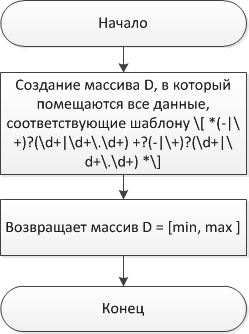
\includegraphics{getPointData.png}}
\caption{Блок-схема функции получения массива значений для графиков}
\label{ris:image}
\end{figure}
\subsection{Создание\enspaceшкалы\enspaceдля\enspaceграфиков}
\hspace{4ex}При вызове данной функции происхоит поиск минимального и максимального значения графика, рисуются шкалы и возвращается функции, для шкал.
\newpage
\begin{figure}[h]
\center{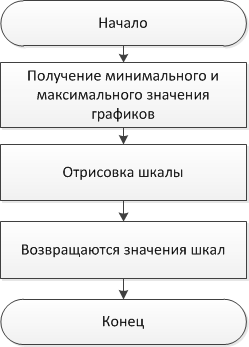
\includegraphics{createNumericScales.png}}
\caption{Блок-схема функции создания шкалы для графиков}
\label{ris:image}
\end{figure}
\subsection{Отрисовка\enspaceточек\enspaceна\enspaceграфике}
\hspace{4ex}Данная функция отрисовывает точки на графике с учетом данных, переданных функции и шкалы для определения положения точки на графике. Точки рисовались с помощью SVG элемента \textit{circle} с радиусом в 3 пикселя.
\hspace{4ex}Данная функция также предусматривает показ координат точки с помошью всплываюшей подсказки (tooltip).
\begin{verbatim}
d3.select(this).on("mouseenter", function() {
    element.select('.tip').attr('class', 'tip vis')
        .style('top', (scales.yScale(d[1])) + 'px')
        .style('left', scales.xScale(d[0]) + 'px');
    element.select('.tip').select('.s').text('Serie: point');
    element.select('.tip').select('.p')
        .text('X: ' + d[0] + ', Y:' + d[1]);
})
d3.select(this).on("mouseleave", function() {
    element.select('.tip').attr('class', 'tip');
})
\end{verbatim}
\newpage
\begin{figure}[h]
\center{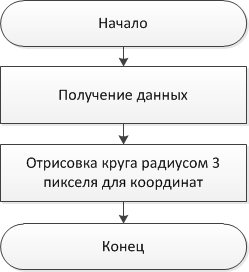
\includegraphics{point.png}}
\caption{Блок-схема функции отрисовки точек на графике}
\label{ris:image}
\end{figure}
\subsection{Отрисока\enspaceломанных\enspaceлиний\enspaceи\enspaceсплайнов\enspaceна\enspaceграфике}
\hspace{4ex}При вызове данной функции на графике появляются ломанные линии, узлы которых задаются разработчиком в html-документе и в последствии преобразовываются в массив координат.\\
\hspace{4ex}Данная функция способна преобразовать ломанные линии в плавные линии (сплайны). Для этого в параметры функции необходимо пятым параметром передать значение \textit{true}.
\begin{verbatim}
var line = d3.svg.line()
    .x(function(d) {
        return scales.xScale(d[0]);
    })
    .y(function(d) {
        return scales.yScale(d[1]);
    })
if (spline) {
    line.interpolate("basis");
}
element.select('svg').append('path')
    .attr('d', line(v))
    .attr('stroke', colors[i])
    .attr('stroke-width', 2)
    .attr('fill', 'none')
i++;
\end{verbatim}
\hspace{4ex}Также функция отрисовки линий, как и функция рендеринга точек, при наведении курсором мышки на линию появится всплывающая подсказка о текущих координатах точки графика.
\subsection{Отрисока\enspaceкруговой\enspaceдиаграммы}
\hspace{4ex}Отображение круговой диаграммы производится с помошью функции библиотеки D3.js. Для этого необходимо полученным данным из html-документа присвоить метку \textit{d3.layout.pie()}.\\
\begin{figure}[h]
\center{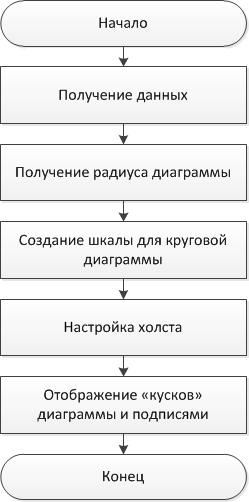
\includegraphics{pie.png}}
\caption{Блок-схема функции отображения круговой диаграммы}
\label{ris:image}
\end{figure}
\hspace{4ex}При наведение курсора мышки на диаграмму, остается подсвеченной только та её часть, внутри которой находится указатель.
\end{document}